\documentclass[12pt, letterpaper]{article}

% --- Packages ---
\usepackage{geometry}
 \geometry{margin=1in}
\usepackage{graphicx}
\usepackage{amsmath, amssymb}
\usepackage{booktabs}
\usepackage{hyperref}
\usepackage{cite}
\usepackage{setspace}
\onehalfspacing
\usepackage{fontspec}
\usepackage{polyglossia}
\usepackage{float}
\usepackage{svg}
\setmainlanguage{vietnamese}

\usepackage{listings}
\usepackage{xcolor}

\lstset{
    language=C,
    basicstyle=\ttfamily\small,
    keywordstyle=\color{blue},
    stringstyle=\color{red},
    commentstyle=\color{green!60!black},
    breaklines=true,
    frame=single, % Tạo khung xung quanh code
    backgroundcolor=\color{gray!5}
}

\renewcommand{\lstlistingname}{Mã nguồn}

% --- Metadata ---
\title{Tạo cây tiến trình cho chương trình bài tập 3}
\author{Đỗ Hoàng Gia Bảo - 23020783 \\ \small Khoa Điện tử - Viễn Thông}
\date{\today}

\begin{document}

\maketitle

\begin{abstract}
Báo cáo sẽ trình bày các bước vẽ ra cây tiến trình chứa tiến trình chạy chương trình trong "Bài tập 3" và các tiến trình sinh ra bởi các lệnh fork(), hiển thị pid của mỗi tiến trình trong cây, số lượng tiến trình trong cây tiến trình.
\end{abstract}
% --- Front Matter (Roman Numerals) ---
\newpage
\tableofcontents

% --- Main Content (Arabic Numerals) ---
\newpage
\pagenumbering{arabic}
\setcounter{page}{3} % This automatically resets the counter to 1

\section{Yêu cầu bài tập}
Bài tập 3 cho một chương trình như sau:

\begin{lstlisting}[language=C, caption={Nội dung file C của bài tập}, label={lst:main}]
#include <stdio.h>
#include <unistd.h>
int main()
{
    int i;
    int N=10;

    for (i = 0; i < N; i++)
            fork();
    return 0;
}
\end{lstlisting}

\noindent Khi chạy chương trình trên, vòng lặp for sẽ chạy 10 lần, mỗi lần đều gọi hàm hệ thống "fork()". Mỗi lần gọi hàm này, số lượng tiến trình tăng lên gấp đôi. Vì ta gọi "fork()" 10 lần trong vòng lặp, chương trình trên sẽ tạo ra $2^{10}$ tiến trình hay 1024 tiến trình.\\
Nhiệm vụ của bài tập là phải biểu diễn được tất cả các tiến trình tạo ra từ chương trình trên thành một kiểu cây tiến trình để thể hiện mối quan hệ của các tiến trình. Cần in ra số lượng tiến trình và mỗi tiến trình cần phải in ra số hiệu tiến trình (PID) của chúng.

\section{Các bước giải quyết bài toán}
\subsection{Phát hiện tiến trình cha và tiến trình con}
Hàm hệ thống fork() tạo ra một bản sao của tiến trình hiện tại. Giá trị trả về của fork() là chìa khóa để phân biệt:
\begin{itemize}
\item Giá trị bằng 0: Tiến trình đang chạy là tiến trình con (child process).
\item Giá trị lớn hơn 0: Tiến trình đang chạy là tiến trình cha (parent process), và giá trị trả về chính là PID của con nó.
\item Giá trị âm: Lỗi xảy ra, không có tiến trình mới nào được tạo.
\end{itemize}

\subsection{Thuật toán xây dựng cây tiến trình}
Để in ra cây tiến trình và số lượng tiến trình một cách chính xác, chúng ta cần sửa đổi mã nguồn gốc. Thay vì chỉ gọi fork() và kết thúc, mỗi tiến trình cần:
\begin{itemize}
\item Lưu trữ thông tin: Sử dụng một mảng hoặc cấu trúc dữ liệu để ghi lại mối quan hệ cha-con.
\item Đồng bộ hóa: Tiến trình cha phải chờ (wait()) các tiến trình con kết thúc để đảm bảo cây được in ra đầy đủ và không bị "mồ côi" (orphan process).
\item Đệ quy: Cấu trúc cây được hình thành tự nhiên theo mô hình nhị phân. Với $N=10$, tổng số tiến trình sẽ là $2^{10} = 1024$.
\end{itemize}

\subsection{Chỉnh sửa chương trình}
Chương trình được chỉnh sửa như sau để vẽ được cây tiến trình:
\begin{lstlisting}[language=C, caption={Mã nguồn để vẽ được cây tiến trình}]
#include <stdio.h>
#include <unistd.h>
#include <sys/wait.h>
#include <stdlib.h>

int main() {
    int i;
    int N = 10; 
    pid_t root_pid = getpid();

    // .dot file configuration for tree graph
    if (getpid() == root_pid) {
        printf("digraph ProcessTree {\n");
        printf("    rankdir=LR;\n");
        printf("    node [shape=circle, fontsize=10];\n");
    }

    for (i = 0; i < N; i++) {
        pid_t child_pid = fork();

        if (child_pid < 0) {
            perror("fork failed");
            exit(1);
        }

        if (child_pid == 0) {
            // Child process: Print its connection to its parent
            printf("    \"%d\" -> \"%d\";\n", getppid(), getpid());
        } else {
            // Parent process: continues loop to create more children
        }
    }

    // Give processes time to finish printing before the file closes
    usleep(200000); 

    // Only the original root process prints the closing brace
    if (getpid() == root_pid) {
        printf("}\n");
    }

    return 0;
}
\end{lstlisting}

\noindent Sử dụng kiểu dữ liệu và định dạng đồ thị thể hiện trong file .dot, các phần mềm như Graphviz có thể được sử dụng để vẽ cây tiến trình. \\
Sử dụng luồng điều khiển if-else để có thể phân biệt tiến trình con (pid == 0) và tiến trình cha (pid > 0) để thực hiện in mối quan hệ giữa tiến trình con và tiến trình cha. Sau đó, ghi dòng được in này vào file .dot.\\
Để chạy chương trình, ta cần phải biên dịch trước bằng cách nhập lệnh sau vào terminal.
\begin{figure}[H]
    \centering 
    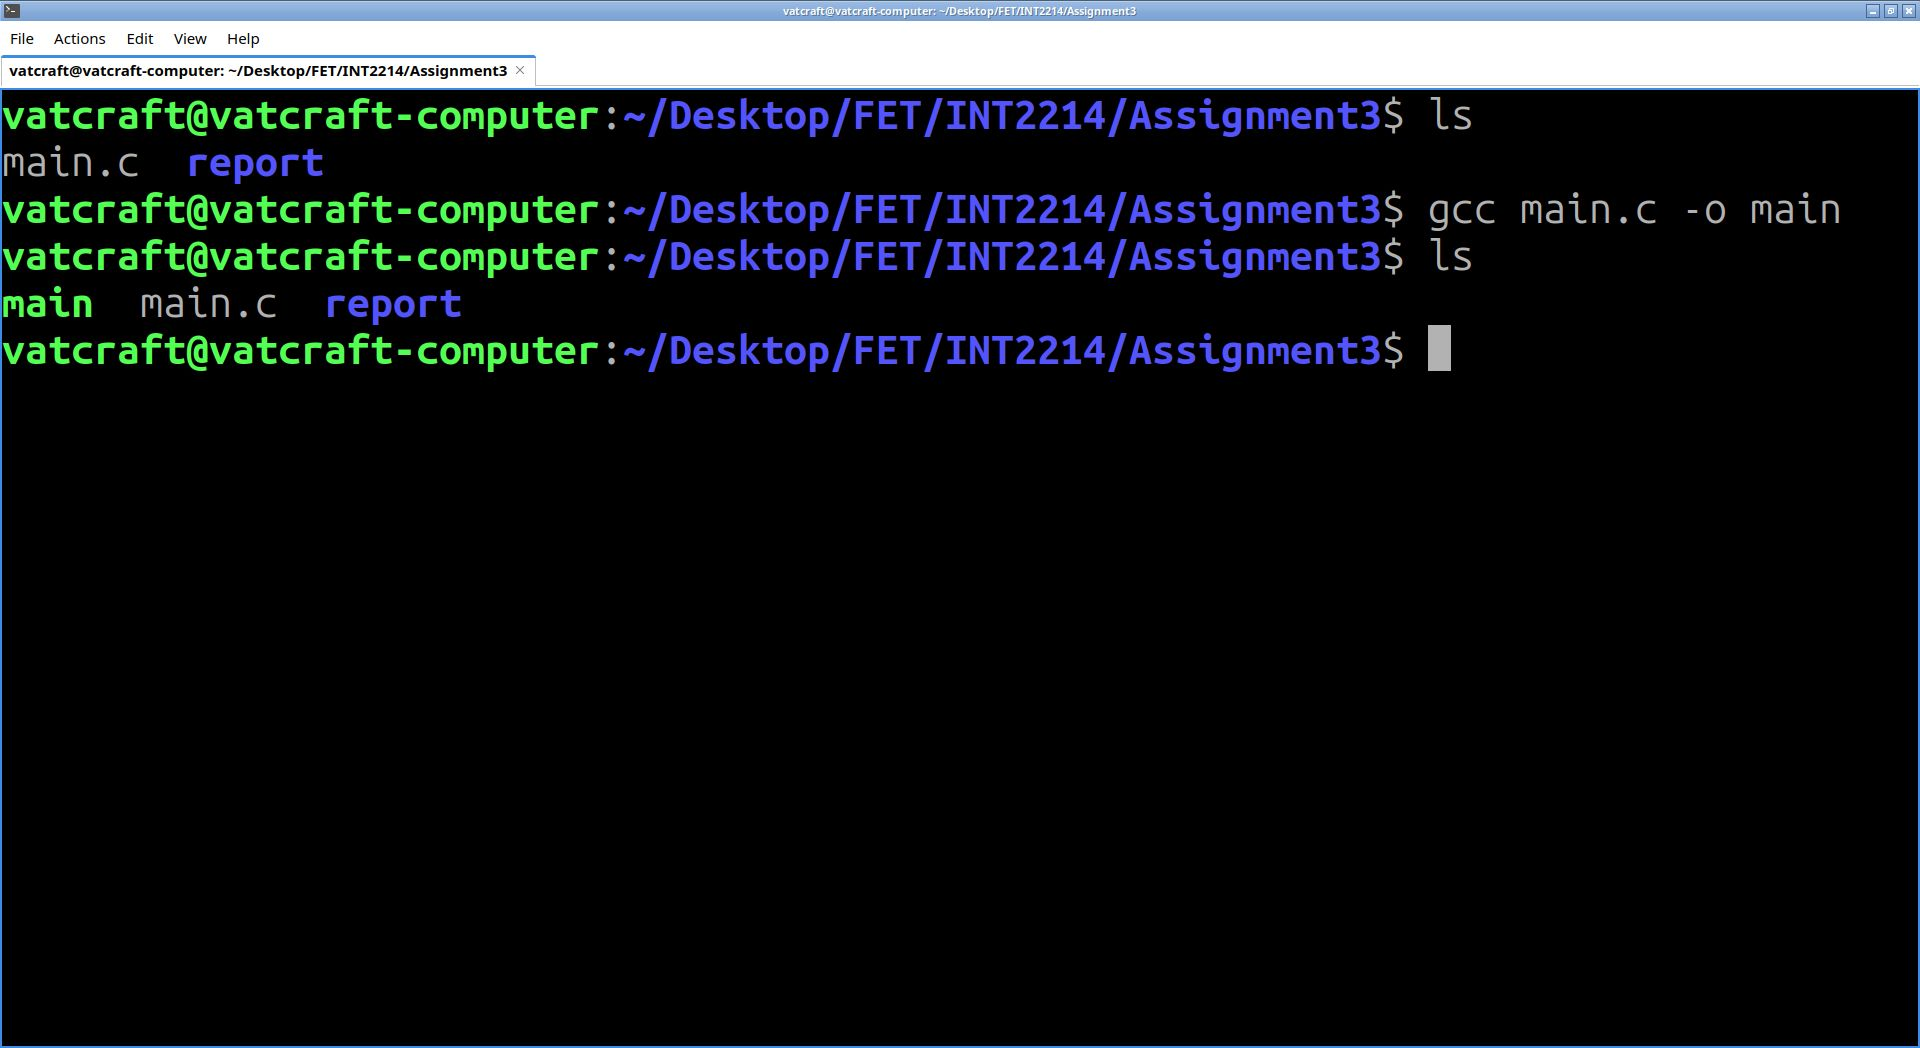
\includegraphics[width=1\textwidth]{screen1.jpg}
    \caption{Lệnh để biên dịch chương trình} 
    \label{fig:screen1} 
\end{figure}

Để có thể  viết .dot file, ta nhập lệnh sau vào terminal.
\begin{figure}[H]
    \centering 
    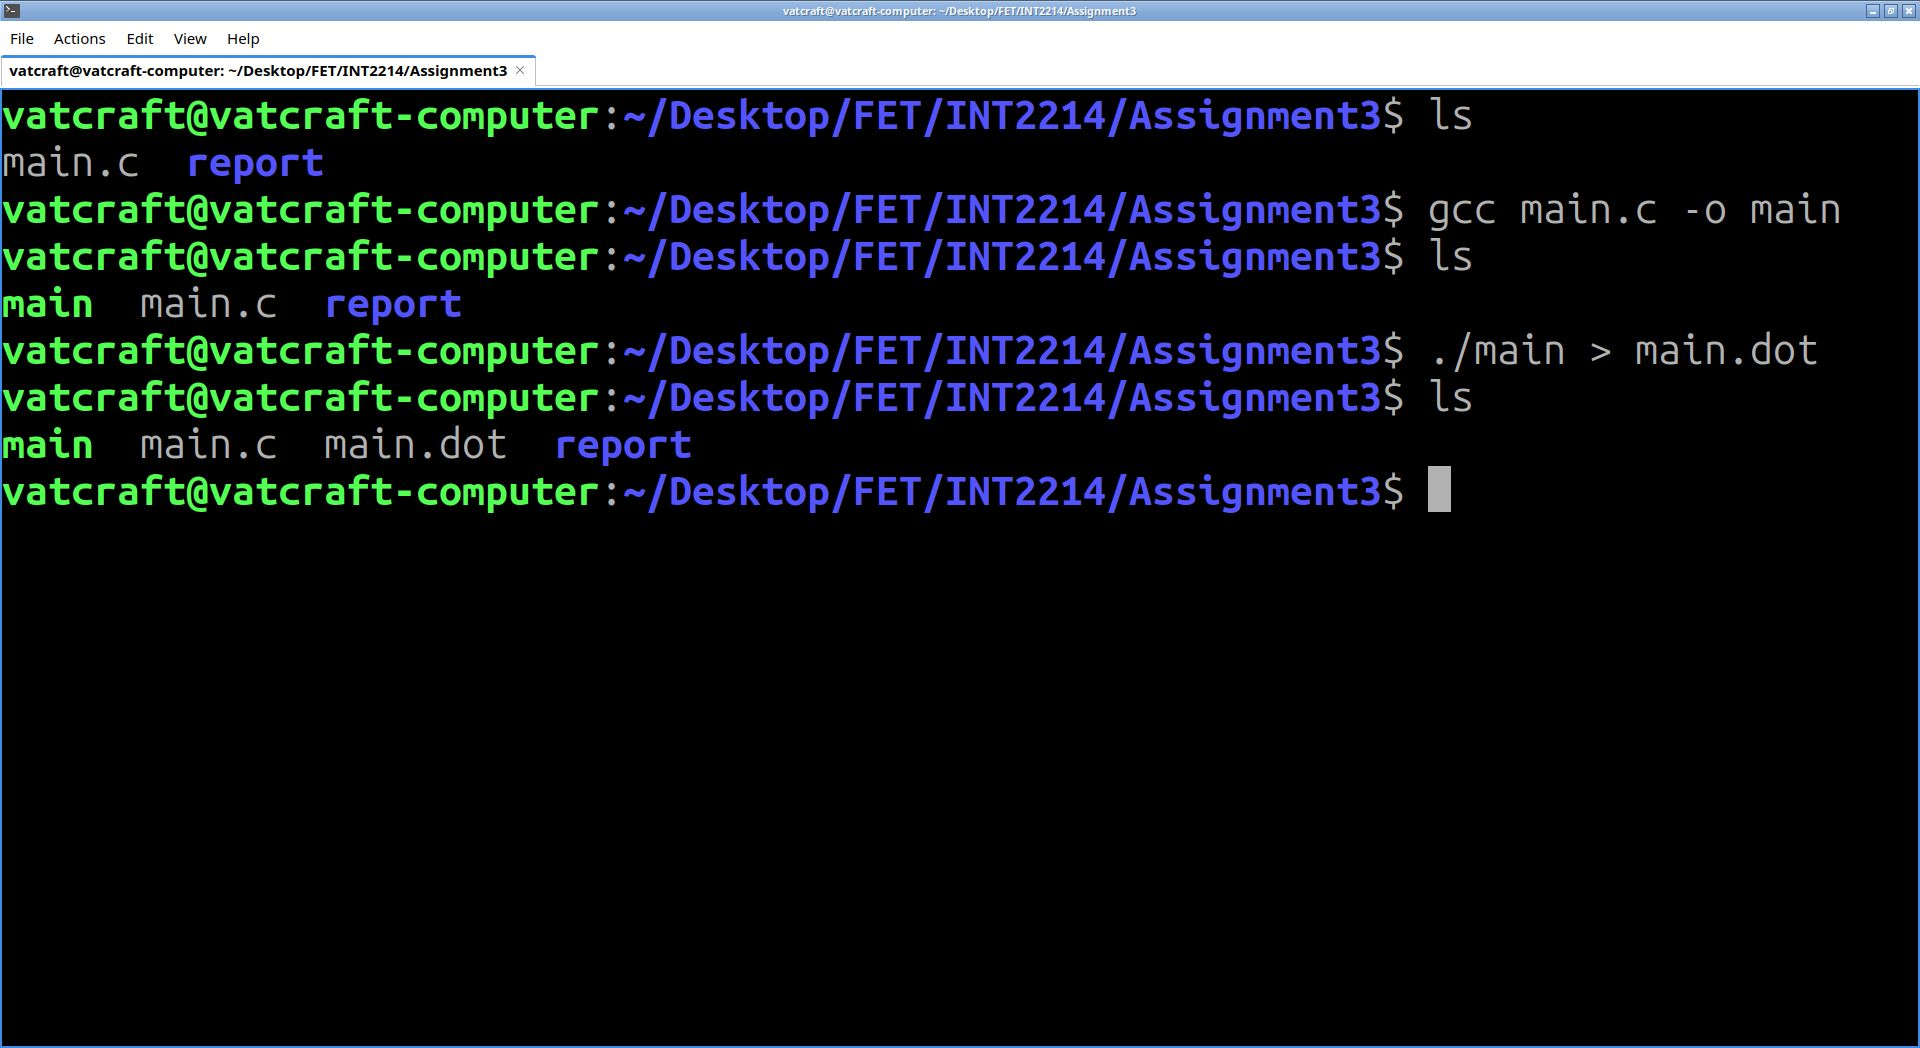
\includegraphics[width=1\textwidth]{screen2.jpg}
    \caption{Tạo file .dot} 
    \label{fig:screen2} 
\end{figure}

Sử dụng phần mềm Graphviz, cây tiến trình được vẽ như sau.
\begin{figure}[H]
    \centering 
    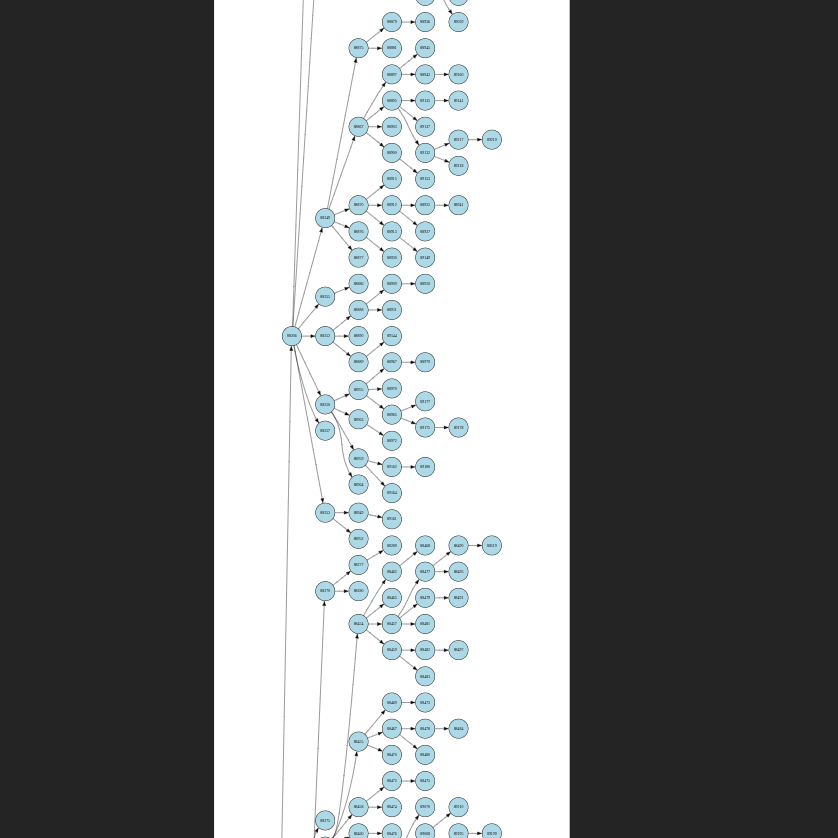
\includegraphics[width=1\textwidth]{image.png}
    \caption{Cây tiến trình sau khi vẽ qua Graphviz} 
    \label{fig:image}
\end{figure}

Để có thể nhìn cây tiến trình rõ ràng hơn, mở file \href{https://drive.google.com/file/d/1XZEyfcf3cVNtKzd7aQQ8j4HVI_pR3K39/view?usp=drive_link}{graphviz.svg} để xem rõ hơn.
\end{document}